% generated by scripts/pkl_to_latex.py
% source PKL : tscan_v1_L6_Ne6_U5_mode-uniform_nmin2_solver-gcg_full_es_restarts10_iter300_kmax5_tol1em09_t0.05to2_N21-32c2aa6cb1ca.pkl
% scan type  : tscan
% state      : ex_singlet
% requires   : \usepackage{pgfplots} \pgfplotsset{compat=1.18}
% colours match the matplotlib PDF (tab10 cycle)
\definecolor{gmeC0}{HTML}{1F77B4}
\definecolor{gmeC1}{HTML}{FF7F0E}
\definecolor{gmeC2}{HTML}{2CA02C}
\definecolor{gmeC3}{HTML}{D62728}
\definecolor{gmeC4}{HTML}{9467BD}
\definecolor{gmeC5}{HTML}{8C564B}
\definecolor{gmeC6}{HTML}{E377C2}
\definecolor{gmeC7}{HTML}{17BECF}

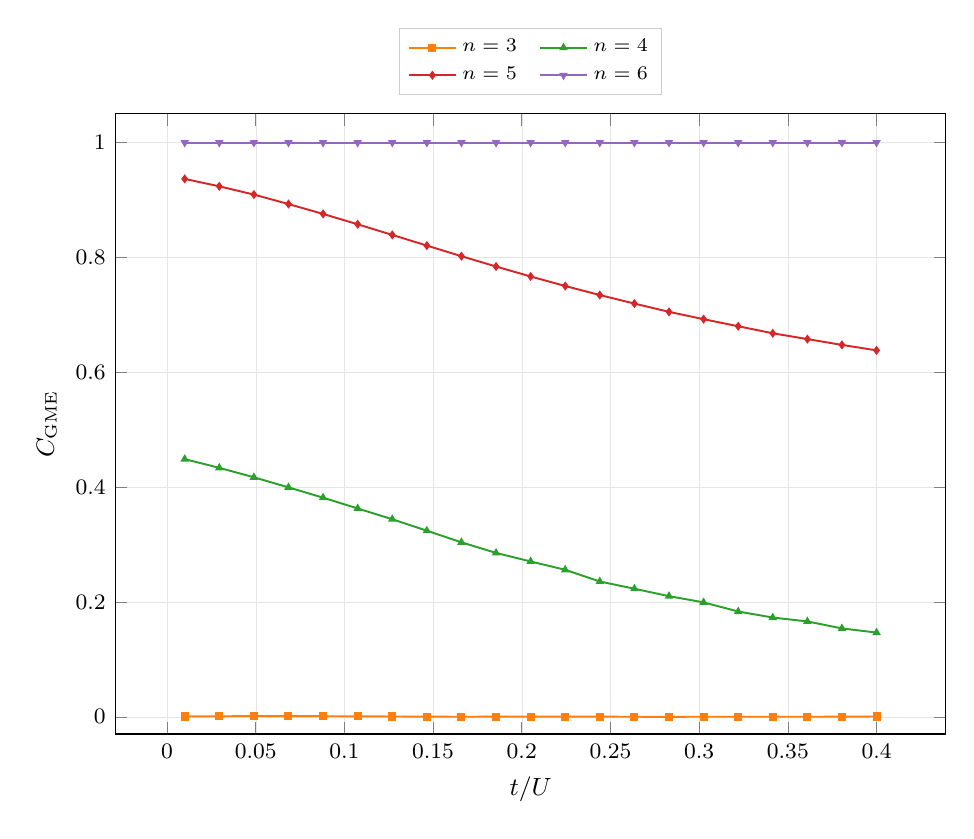
\begin{tikzpicture}
  \begin{axis}[
    width=\columnwidth,
    height=0.78\columnwidth,
    xlabel={$t/U$},
    ylabel={$C_{\mathrm{GME}}$},
    grid=both,
    grid style={line width=.1pt, draw=gray!20},
    tick label style={font=\footnotesize\rmfamily, /pgf/number format/fixed},
    label style={font=\small\rmfamily},
    scaled ticks=false,
    legend style={font=\scriptsize\rmfamily, draw=gray!40, at={(0.5,1.03)}, anchor=south, /tikz/every even column/.append style={column sep=6pt}},
    legend cell align={left},
    legend columns=2,
    ymin=-0.03,
    ymax=1.05,
  ]
    \addplot[color=gmeC1, mark=square*, mark size=1.1pt, line width=0.7pt] coordinates {
        (0.01,0.000555) (0.0295,0.000793) (0.049,0.001412) (0.0685,0.001195)
        (0.088,0.00107) (0.1075,0.000751) (0.127,0.000555) (0.1465,0.000314)
        (0.166,0.00007) (0.1855,0.000261) (0.205,0.000227) (0.2245,0.000158)
        (0.244,0.000278) (0.2635,0.000055) (0.283,0.000017) (0.3025,0.000082)
        (0.322,0.000062) (0.3415,0.000153) (0.361,0.000039) (0.3805,0.000283)
        (0.4,0.000531)
    };
    \addlegendentry{$n=3$}
    \addplot[color=gmeC2, mark=triangle*, mark size=1.1pt, line width=0.7pt] coordinates {
        (0.01,0.448737) (0.0295,0.433564) (0.049,0.417155) (0.0685,0.399546)
        (0.088,0.381581) (0.1075,0.362808) (0.127,0.344074) (0.1465,0.324087)
        (0.166,0.303844) (0.1855,0.285377) (0.205,0.270542) (0.2245,0.255981)
        (0.244,0.235622) (0.2635,0.223028) (0.283,0.210096) (0.3025,0.199271)
        (0.322,0.183369) (0.3415,0.172845) (0.361,0.166078) (0.3805,0.153936)
        (0.4,0.146686)
    };
    \addlegendentry{$n=4$}
    \addplot[color=gmeC3, mark=diamond*, mark size=1.1pt, line width=0.7pt] coordinates {
        (0.01,0.93675) (0.0295,0.923798) (0.049,0.909411) (0.0685,0.892933)
        (0.088,0.875733) (0.1075,0.857702) (0.127,0.839197) (0.1465,0.82057)
        (0.166,0.802134) (0.1855,0.784146) (0.205,0.766796) (0.2245,0.750212)
        (0.244,0.734468) (0.2635,0.719596) (0.283,0.705203) (0.3025,0.692455)
        (0.322,0.680131) (0.3415,0.667861) (0.361,0.657771) (0.3805,0.647639)
        (0.4,0.638143)
    };
    \addlegendentry{$n=5$}
    \addplot[color=gmeC4, mark=triangle*, mark size=1.1pt, mark options={rotate=180}, line width=0.7pt] coordinates {
        (0.01,1) (0.0295,1) (0.049,1) (0.0685,1)
        (0.088,1) (0.1075,1) (0.127,1) (0.1465,1)
        (0.166,1) (0.1855,1) (0.205,1) (0.2245,1)
        (0.244,1) (0.2635,1) (0.283,1) (0.3025,1)
        (0.322,1) (0.3415,1) (0.361,1) (0.3805,1)
        (0.4,1)
    };
    \addlegendentry{$n=6$}
  \end{axis}
\end{tikzpicture}
